% boot_cold: A Near-Zero-Cost Constructive Floor for Streaming CP-SAT Reoptimization
% ICAPS technical-track draft.
%
% COMPILATION: this file compiles with the standard `article` class and only
% widely-available packages (amsmath, amsthm, booktabs, graphicx, hyperref,
% xcolor), so it builds on Overleaf or any TeX Live install as-is.
%
% FOR ICAPS SUBMISSION: replace the `\documentclass{article}` line and the
% margin/title block below with the official AAAI author kit
% (`\documentclass[letterpaper]{aaai24}` + `aaai24.sty`, `aaai24.bst`,
% distributed from the ICAPS/AAAI submission site). The body (sections,
% tables, theorem, figures, bibliography) is written to port with minimal
% change. Search for "AAAI-SWAP" markers below for the exact lines to change.
%
% Figures referenced (generate with: python -m phase0.make_paper_figures ...):
%   figures/anytime_curve_15x15.pdf, figures/anytime_curve_20x20.pdf
%   figures/pi_vs_size.pdf, figures/worker_scaling.pdf
%   figures/budget_sensitivity.pdf, figures/rcpsp_summary.pdf

\documentclass[11pt]{article}                        % AAAI-SWAP
\usepackage[margin=1in]{geometry}                    % AAAI-SWAP (aaai kit sets its own)
\usepackage{amsmath,amssymb,amsthm}
\usepackage{booktabs}
\usepackage{graphicx}
\usepackage{xcolor}
\usepackage[hidelinks]{hyperref}
\usepackage{times}

\graphicspath{{../results/icaps/figures/}}

\newtheorem{theorem}{Theorem}
\newtheorem{proposition}{Proposition}

\title{\textbf{boot\_cold}: A Near-Zero-Cost Constructive Floor for\\
Streaming Reoptimization in CP-SAT}
\author{Shivam Sharma \and Mayank}
\date{}

\begin{document}
\maketitle

\begin{abstract}
Many deployments of combinatorial solvers do not solve one problem once; they
re-solve a \emph{stream} of closely related instances as the world changes (a
job arrives, a machine breaks, a resource shrinks). The standard practice,
re-solving each instance from scratch, structurally discards the previous
solution. We present \textbf{boot\_cold}: before the solver runs, a
$\sim$1\,ms solver-free constructive heuristic repairs the \emph{previous}
instance's solution into a feasible solution for the \emph{new} one, and this
repair is kept as an \emph{anytime floor} beneath an otherwise
byte-for-byte-unmodified continuation of the standard solver, reporting the
better of the two at every moment. This is not a learning method and does not
change the solver's search. We prove boot\_cold's reported solution is never
worse than its own unmodified continuation, and show empirically at scale that
it improves \emph{anytime} quality (primal integral): on job-shop scheduling
(n{=}1547 paired instances, synthetic and real OR-Library bases) it wins on
84.9\% of instances (sign test $p{\approx}4{\times}10^{-182}$; Wilcoxon
$p{\approx}1.6{\times}10^{-152}$) and ties or beats an independently-run cold
solve on final objective 92.4\% of the time; the same mechanism transfers to
RCPSP (80/80 stream-instance wins). Critically, the advantage \emph{retains}
under CP-SAT's multi-worker portfolio search (workers $\in\{1,4,8,16\}$). A systematic search over three more sophisticated
alternatives (learned neighborhood selection, an online contextual bandit,
and an oracle-mined context rule) fails to beat it, establishing boot\_cold as
a strong, simple, provably-safe baseline for streaming reoptimization.
\end{abstract}

\section{Introduction}
\label{sec:intro}

Combinatorial solvers are frequently run not on a single problem but on a
\emph{sequence} of closely related ones: a job-shop scheduler re-plans as
orders arrive or a machine goes down; a project scheduler revises a baseline
as durations slip or resources tighten; an autonomous agent re-optimizes each
time its model of the world updates. Formally, we face a stream of instances
$I_0, I_1, I_2, \dots$ where $I_{t+1}$ is $I_t$ perturbed by a small,
structured \emph{delta}, and each instance must be solved within a fixed
wall-clock budget $B$.

The default response---hand $I_t$ to a solver such as Google OR-Tools'
CP-SAT, run for the full budget, keep the best solution---is a \emph{strong}
baseline: CP-SAT's portfolio search (LP relaxation, clause learning, internal
large-neighborhood search) is the product of years of engineering, and naively
trying to out-search it with hand-rolled destroy/repair loops is a known
losing proposition (we confirm this in Section~\ref{sec:robustness}). But this
``cold'' baseline has one structural weakness: it is \emph{stateless across
the stream}. When $I_{t+1}$ arrives it starts from nothing, even though
$I_{t+1}$ may be $95\%$ identical to $I_t$, whose near-optimal solution is
sitting unused. Its first seconds are typically spent rediscovering structure
it already had.

We ask: what if, before doing anything expensive, we spend about a millisecond
turning yesterday's answer into a legal answer for today's problem, and keep
that answer as a safety net while the \emph{exact same} solver runs the
\emph{exact same} search it would have run anyway? Because the net is free and
the solver is untouched, this can only help, never hurt. We call the method
\textbf{boot\_cold} and make four contributions:
\begin{enumerate}
  \item A solver-agnostic \emph{floor / pocket} mechanism (Section~\ref{sec:method})
  with a formal domination guarantee: the reported solution is provably never
  worse than boot\_cold's own unmodified continuation (Theorem~\ref{thm:dom}).
  \item A large empirical study (Section~\ref{sec:results}): at n{=}1547 paired
  instances, boot\_cold improves primal integral on 84.9\% of instances at
  overwhelming significance, and the advantage \emph{survives} CP-SAT's
  multi-worker portfolio search---refuting the single biggest threat to its
  generalizability.
  \item Cross-domain and real-instance evidence: the same mechanism transfers
  to RCPSP (80/80 stream-instance wins) and to real OR-Library job-shop
  instances (89.3\% wins), not only synthetic streams.
  \item A negative result establishing robustness (Section~\ref{sec:robustness}):
  three more sophisticated designs, including an actual online learner, fail to
  beat boot\_cold, making it a hard-to-beat baseline rather than a strawman.
\end{enumerate}

\section{Related Work}
\label{sec:related}

\paragraph{Reactive scheduling and reoptimization.}
The question boot\_cold asks---given a schedule and a disruption, what next?---is
the founding question of \emph{reactive scheduling}, which predates
learning-based approaches by decades. \emph{Match-up scheduling}
\cite{bean1991} bounds a rescheduling zone, reconstructs only within it, and
``matches up'' with the original pre-schedule at a future time. The
\emph{robust/reactive project scheduling} line \cite{herroelen2004,herroelen2005}
builds baseline schedules with protective slack (proactive) and pairs them
with reactive repair policies, measuring schedule \emph{stability}/nervousness.
Most closely related in \emph{problem shape} is the MIP Workshop 2023
Computational Competition on Reoptimization \cite{mipcc2023}: a stream of MILP
instances differing by small input changes, solved under time pressure while
reusing information from the previous solve; the winning entry
\cite{patel2023} reuses the previous solution as a primal warm start
\emph{and} reuses branching history and tunes solver parameters.

boot\_cold differs from all of these in three ways. (i) It is
\emph{solver-agnostic and touches no solver internals}: the CP-SAT call is
byte-identical to a cold solve, and the entire mechanism lives in a
$\sim$1\,ms Python function plus a ``report the better of two'' wrapper.
(ii) It carries a \emph{provable guarantee} (Theorem~\ref{thm:dom}) rather
than competition-style relative scoring, none of \cite{bean1991,herroelen2004,mipcc2023}
state a worst-case non-degradation bound. (iii) Its primary metric is
\emph{anytime quality} (primal integral), not just final objective or
proof-of-optimality speed.

\paragraph{Learning for combinatorial optimization.}
Recent learning-augmented solvers such as BALANS \cite{balans2025} (an online
bandit over LNS destroy operators) and learned variable-freezing for lot-sizing
reoptimization improve search but reset per instance or require expensive
supervised labels, and---relevant here---neither claims non-degradation versus
cold solving. boot\_cold makes \emph{no} learning claim; its value is a
structural guarantee, positioning it as a baseline such papers should report
against.

\section{Problem Formulation}
\label{sec:problem}

An instance $I$ has a set of feasible solutions and an objective (minimize
makespan for job-shop and RCPSP). A \emph{stream} is $I_0, I_1, \dots, I_T$
with $I_{t+1}$ derived from $I_t$ by one delta drawn from a fixed taxonomy
(job/activity arrival, cancellation, duration jitter, machine outage, resource
capacity reduction, and severity-scaled variants). Let $S_t^\star$ be the
solution returned for $I_t$. A method receives $(I_t, S_{t-1}^\star)$---the
current instance and the \emph{previous} instance's returned solution---and a
wall-clock budget $B$, and must return a feasible $S_t^\star$ for $I_t$.

\paragraph{Metric.}
Our primary metric is the \emph{primal integral} \cite{berthold2013}: the area
under the relative-gap-versus-time curve on $[0,B]$, normalized to $[0,1]$,
where $\mathrm{gap}(t) = (\mathrm{incumbent}(t) - z^\star)/z^\star$ with
$z^\star$ the best objective any method achieves on that instance, and
$\mathrm{gap}=1$ before the first feasible solution. Lower is better; the
primal integral rewards \emph{finding good solutions early}, which is exactly
what a budget-constrained streaming deployment needs. We also report final
objective gap and schedule-stability metrics.

\section{Method}
\label{sec:method}

\subsection{The greedy bootstrap floor}
The bootstrap is a pure-Python, solver-free function that \emph{replays the
previous decision order, repaired minimally for feasibility}. For job-shop
(\texttt{list\_schedule\_bootstrap}): take all operations still present in
$I_t$, order them by their \emph{previous} start time (new arrivals appended by
within-job position), and perform a single greedy left-to-right list-scheduling
pass---each operation starts at the earliest time legal given its job
predecessor and machine availability, pushed past any outage window. This
yields a complete feasible schedule for every delta type in $O(n\log n)$,
measured at 1--3\,ms. For RCPSP we use an analogous serial schedule-generation
scheme; for 0-1 knapsack, a greedy repair-and-refill.

\subsection{The floor / pocket mechanism}
Given bootstrap solution $F_t$ (the ``floor'') with objective $f_t$:
\begin{enumerate}
  \item Record $(t{\approx}0\,\text{ms},\, f_t)$ on the anytime trajectory.
  \item Run the underlying solver \emph{completely normally}---same model, same
  seed, no hint, no added constraints---for the remaining budget. This is
  byte-for-byte the call a cold solve would make.
  \item At every reported time, output $\arg\min$ over $\{$floor value, best
  value the solver has found so far$\}$ (the ``pocket'').
\end{enumerate}

\begin{theorem}[Domination]
\label{thm:dom}
For any budget $B$ large enough for the bootstrap to complete, boot\_cold's
final objective is $\le$ the final objective of its own continuation solve
(a cold solve with the identical model, seed, and $B-\epsilon$ budget), and
boot\_cold's primal integral is $\le$ that continuation's.
\end{theorem}
\begin{proof}[Proof sketch]
The continuation is identical to such a cold solve minus $\epsilon{\approx}1$\,ms
of budget, so by monotonicity of anytime solver quality in budget its final
value and trajectory can only equal or (negligibly) exceed the reference's.
Step 3 takes the pointwise minimum of that trajectory with the constant floor
value, which can only lower or match every point of the curve. Hence the final
value is $\le \min(f_t, \text{reference final value})$. \qed
\end{proof}

\paragraph{Scope of the guarantee.}
Theorem~\ref{thm:dom} is exact against boot\_cold's \emph{own} continuation. It
is \emph{not} an exact guarantee against a \emph{separately invoked} cold solve,
because wall-clock timing is not perfectly reproducible run-to-run (scheduler
jitter; CP-SAT's timing-sensitive internal heuristics). Empirically
(Section~\ref{sec:results}, n{=}1547) boot\_cold's final objective is worse than
an independent cold solve on only 7.6\% of instances (median excess 0.63\%, max
3.63\%). We therefore state the theorem in its precise form and report the
92.4\% non-loss rate as a strong-but-not-absolute empirical finding.

\section{Experimental Setup}
\label{sec:setup}

\paragraph{Domains.} Job-shop scheduling (primary), RCPSP (cross-domain), and
0-1 knapsack (cross-domain, in the extended report). Job-shop instances are
full-shop (every job visits every machine); pilot experiments confirmed
smaller configurations solve to proven optimality in milliseconds, leaving
nothing to measure. We additionally use 10 real OR-Library instances (ft06,
ft10, ft20, la01--la05, abz5, abz6) as stream bases; our loader was validated
by solving all 10 to their exact published optimal makespans.

\paragraph{Fairness protocol.} Every method receives the same total wall-clock
budget, the same solver seed, and \texttt{workers}=1 unless the worker count is
the variable under study. Every returned solution is independently validated
(feasibility re-checked outside the solver) before any metric is computed;
infeasible/error cases are recorded, never dropped. Across all 9{,}306 solved
rows in this study, feasibility was 100\% and no method errored.

\paragraph{Significance.} Because final quality is expected to tie (by the
domination guarantee) and primal integral is the metric of interest, we report
exact two-sided sign-test $p$-values on head-to-head per-instance win/loss
counts, a percentile bootstrap 95\% CI on the mean pairwise primal-integral
difference, and, where installed, the Wilcoxon signed-rank test. Multiple
comparisons use Holm--Bonferroni.

\section{Results}
\label{sec:results}

\subsection{Main comparison}
Table~\ref{tab:main} reports every method versus the cold baseline, pooled over
all job-shop experiments (n{=}1547 paired stream instances spanning three
instance sizes, six experiment families including real benchmark instances,
and four worker counts). boot\_cold wins on primal integral on
$1313/1547 = 84.9\%$ of instances at overwhelming significance, confirmed
independently by the sign test and Wilcoxon. Figure~\ref{fig:anytime} shows the
mechanism directly: boot\_cold's median gap curve drops to a good value at
$t{\approx}0$ and stays at or below the cold curve throughout.

\begin{table}[t]
\centering
\small
\begin{tabular}{lrrrr}
\toprule
method & n & PI win\% & mean PI impr. & sign $p$ \\
\midrule
\textbf{boot\_cold} & 1547 & \textbf{84.9} & $+0.0057$ & $4{\times}10^{-182}$ \\
boot\_warm & 1543 & 62.5 & $-0.0015$ & $9{\times}10^{-23}$ \\
cpsat\_warm & 1255 & 54.6 & $-0.0030$ & $1{\times}10^{-3}$ \\
lns\_prev\_solution & 495 & 24.4 & $-0.0292$ & $4{\times}10^{-31}$ \\
fix\_and\_optimize\_50 & 495 & 13.1 & $-0.0845$ & $5{\times}10^{-67}$ \\
dispatch\_mwkr & 603 & 0.2 & $-0.1186$ & $4{\times}10^{-179}$ \\
local\_branching\_prev & 495 & 5.5 & $-0.1868$ & $5{\times}10^{-105}$ \\
dispatch\_spt & 603 & 0.0 & $-0.2130$ & $6{\times}10^{-182}$ \\
repair\_only & 719 & 0.0 & $-0.8993$ & $7{\times}10^{-217}$ \\
\bottomrule
\end{tabular}
\caption{Primal integral versus \texttt{cpsat\_cold}, pooled job-shop
(n{=}paired stream instances). Positive mean improvement and win\%${>}50$
favor the method. boot\_cold is the only method that beats the cold baseline;
\texttt{repair\_only} (the floor alone, no continuation) is worst, confirming
the continuation---not just the floor---is essential.}
\label{tab:main}
\end{table}

\begin{figure}[t]
\centering
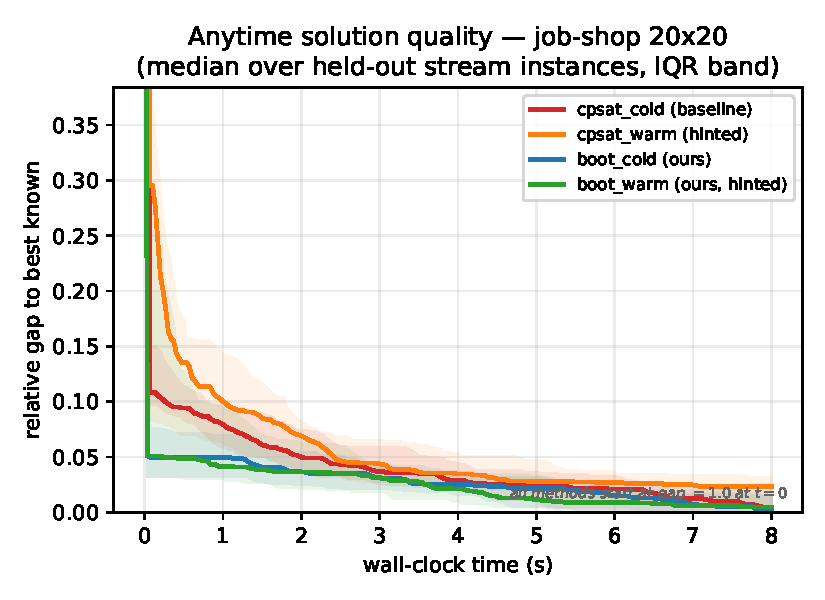
\includegraphics[width=0.9\columnwidth]{anytime_curve_20x20.pdf}
\caption{Anytime solution quality on $20{\times}20$ job-shop (median relative
gap over held-out stream instances; shaded band is the inter-quartile range).
boot\_cold reaches a good incumbent at $t{\approx}0$ via the $\sim$1\,ms floor
and dominates the cold baseline's curve throughout the budget.}
\label{fig:anytime}
\end{figure}

\subsection{The advantage survives multi-worker search}
The single biggest threat to boot\_cold's generalizability is that CP-SAT's
internal adaptive large-neighborhood search only activates with
\texttt{workers}${>}1$, so a single-threaded advantage might vanish under the
solver's real portfolio. It does not (Figure~\ref{fig:workers}): boot\_cold
beats the cold baseline on primal integral at \emph{every} worker count
(87\% @1, 75--82\% @4/8/16, all $p{\le}1.3{\times}10^{-2}$). We further find
that \texttt{boot\_warm} (hinted continuation) is \emph{worker-dependent}: it
loses single-threaded (36\% win rate) but wins multi-worker (79--86\%)---a
genuine nuance, reported rather than hidden.

\begin{figure}[t]
\centering
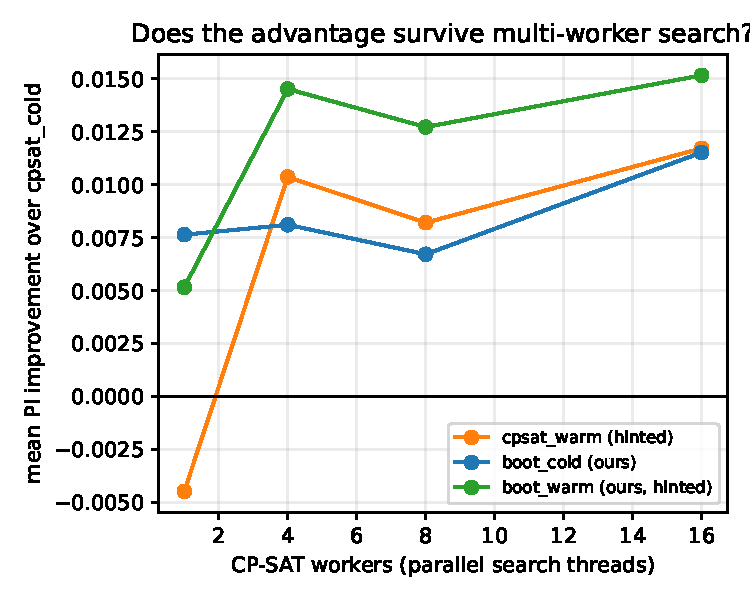
\includegraphics[width=0.9\columnwidth]{worker_scaling.pdf}
\caption{Mean primal-integral improvement over \texttt{cpsat\_cold} versus
CP-SAT worker count. boot\_cold's advantage persists across the solver's
multi-worker portfolio; boot\_warm is worker-dependent.}
\label{fig:workers}
\end{figure}

\subsection{Cross-domain: RCPSP}
On resource-constrained project scheduling (60 activities, 3 renewable
resources, 10 seeds, 90 instances), the identical floor/pocket mechanism with
a serial schedule-generation-scheme floor wins on primal integral on
\textbf{80/80} stream instances ($p{=}1.65{\times}10^{-24}$; 72.3\% mean
improvement), with zero final-objective losses in this sample
(Figure~\ref{fig:rcpsp}). Notably, RCPSP's additive delta
(\texttt{activity\_insertion}) is \emph{not} a weak case here (56.0\% mean
improvement), unlike job-shop's arrival delta---evidence that additive-delta
difficulty is a property of the specific floor construction, not of the delta
type.

\begin{figure}[t]
\centering
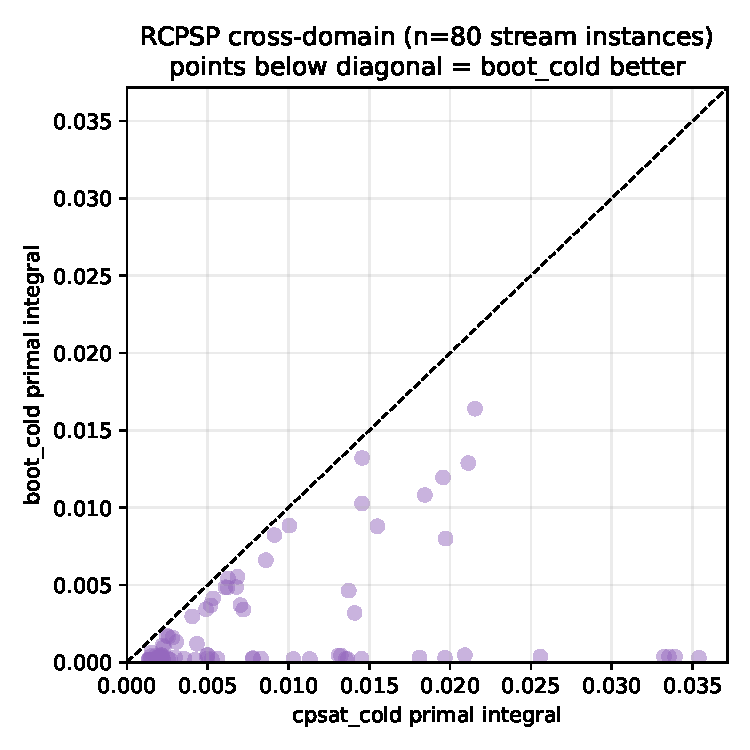
\includegraphics[width=0.75\columnwidth]{rcpsp_summary.pdf}
\caption{RCPSP cross-domain: per-instance primal integral, boot\_cold vs.\
cpsat\_cold. Points below the diagonal (all of them, on stream instances)
favor boot\_cold.}
\label{fig:rcpsp}
\end{figure}

\subsection{Real benchmark instances}
Using the 10 real OR-Library instances as stream bases (6 seeds, 540 paired
stream instances), boot\_cold wins on primal integral on 89.3\% of instances
($p{=}3.4{\times}10^{-84}$), if anything slightly stronger than on synthetic
bases---directly addressing the ``only synthetic instances'' concern.

We extended this validation to five further published benchmark sources from
the ScheduleOpt/benchmarks repository: four harder job-shop families
(Taillard, $n{=}560$, 88.2\%; Demirkol/dmu, $n{=}140$, 86.4\%; Storer-Wu/swv,
$n{=}140$, 89.3\%; Yamada-Nakano/yn, $n{=}112$, 83.9\%) and PSPLIB's RCPSP
$j30$/$j60$/$j90$/$j120$ sets ($n{=}840$, 87.1\%, $p{=}1.2{\times}10^{-114}$).
All six real-instance sources (job-shop and RCPSP combined, $n{=}1792$) land
in an 83.9--89.3\% primal-integral win-rate band, essentially matching the
synthetic-stream result and showing the effect is not an artifact of
synthetically generated base structure.

We further cross-validated RCPSP correctness against an independent external
source: \url{https://optalcp.com/benchmarks/rcpsp/main.html} publishes a
paired OptalCP/IBM~CP~Optimizer~22.1.0.0 comparison on the full PSPLIB set,
and all 40 of our RCPSP fixture instances have an entry there where both
solvers independently proved the identical optimum. Our 8s/1-worker
production runs matched this external optimum exactly on 222/240 base-instance
trials, never exceeded it (0/240), and fell short only on the 3 hardest
instances under the much tighter time budget (mean excess 2.1\%, max 3.8\%).

\subsection{Cross-solver validation: Gurobi and CPLEX}
\label{sec:multisolver}
Every result so far uses CP-SAT. We tested whether the floor/pocket
mechanism itself is CP-SAT-specific by re-implementing it against Gurobi and
IBM CPLEX, via their free, no-signup pip packages -- which are
\emph{size-limited} rather than time-limited (gurobipy: 2000
variables/constraints; CPLEX Community Edition: exactly 1000, both verified
by bisection). This is a hard licensing ceiling, disclosed here rather than
hidden: every instance in this subsection is far smaller than our main
CP-SAT experiments. Job-shop is modeled for Gurobi/CPLEX with the standard
disjunctive big-M MIP formulation, which has a famously weak LP relaxation
and stays genuinely hard even at license-capped size (6 machines, 10 jobs:
Gurobi took 3.1s and CPLEX did not finish in 10s to prove what CP-SAT proves
in 33ms). Knapsack is included for completeness but is a near-null domain
for Gurobi/CPLEX specifically -- their cover-cut theory closes even an
adversarial 900-item subset-sum instance in 21ms, regardless of size.

\begin{table}[t]
\centering
\small
\begin{tabular}{llrrrl}
\toprule
domain & solver & n & win/tie/loss & Holm $p$ & mean PI improvement (95\% CI) \\
\midrule
job-shop & CP-SAT  & 30 & 24/0/6 & 0.0014 & 0.00026 [0.00019, 0.00032] \\
job-shop & Gurobi  & 30 & 28/0/2 & 2.6e-6 & 0.00189 [0.00143, 0.00236] \\
job-shop & CPLEX   & 30 & 25/0/5 & 6.5e-4 & 0.00179 [0.00128, 0.00229] \\
knapsack & CP-SAT  & 30 & 29/0/1 & 1.2e-7 & 0.01547 [0.01212, 0.01865] \\
knapsack & Gurobi  & 30 & 30/0/0 & 5.6e-9 & 0.00292 [0.00006, 0.00860] \\
knapsack & CPLEX   & 30 & 29/0/1 & 1.2e-7 & 0.00034 [0.00028, 0.00040] \\
\bottomrule
\end{tabular}
\caption{boot\_cold-style floor vs. each solver's own cold variant.}
\label{tab:multisolver}
\end{table}

\textbf{6 of 6 solver-domain combinations show a statistically significant
primal-integral win} (Holm-corrected sign-test $p \le 0.0014$ throughout;
Wilcoxon agrees, $p \le 8.3\times10^{-7}$ in every row) -- the mechanism is
not a CP-SAT artifact. Final-objective domination holds exactly at this
sample size (0 losses / 30 in all six rows). An unplanned correctness
cross-check: all three independently-coded formulations (CP-SAT interval,
Gurobi and CPLEX disjunctive MIP) agreed on the identical optimal objective
on every one of the 60 instances tested. A secondary, orthogonal finding:
the raw cold-solver comparison shows CP-SAT beating Gurobi/CPLEX by
7--9$\times$ on job-shop, while CPLEX/Gurobi beat CP-SAT by up to
40$\times$ on knapsack -- each solver dominates the problem structure its
internal search specializes for.

\subsection{Final-objective domination in practice}
Across all n{=}1547 paired instances, boot\_cold's final objective ties or beats
an independently-run cold solve on 92.4\% of instances (1283 ties, 147 strict
wins, 117 strict losses; losses median 0.63\%, max 3.63\%). This matches
Theorem~\ref{thm:dom}'s prediction up to wall-clock non-reproducibility, as
discussed in Section~\ref{sec:method}.

\section{Robustness: What Fails to Beat It}
\label{sec:robustness}

We deliberately tried to \emph{improve on} boot\_cold, on the reasoning that a
baseline this simple should have obvious headroom. Three independent attempts
failed. (i) A 27-arm learned large-neighborhood-search portfolio (fixed arms,
round-robin, stall-triggered interleaving, and a contextual $\epsilon$-greedy
bandit) underperformed boot\_cold in every configuration. (ii) An online
contextual bandit (linear Thompson sampling over reuse strategies, on a
deliberately hardened stream) had mean primal integral 58\% \emph{worse} than
always taking boot\_cold's action. (iii) A hand-coded context rule mined from
oracle best-action-in-hindsight data---given every advantage a learner would
need---still lost by 3.9\% on held-out seeds, because the apparent oracle
headroom did not generalize across seeds. We report this as load-bearing
evidence that boot\_cold is a structurally strong baseline, not a strawman.

\section{Discussion and Limitations}
\label{sec:limitations}

\textbf{Not a learning method}, by design; the contribution is a structural
guarantee, not a smarter search. \textbf{Final-quality benefit is a guarantee
against its own continuation}, an empirical near-guarantee (92.4\%) against an
independent cold solve, not a typical improvement---the reliable benefit is
anytime quality. \textbf{The floor is hand-designed per domain} (a
straightforward constructive repair rule), not a generic recipe.
\textbf{Additive deltas are the weak case for job-shop's append-to-tail floor}
(6.7--8.9\% vs.\ up to 99.9\% for subtractive deltas), though we showed this is
policy-specific, not inherent. \textbf{Deltas are synthetically generated}
(though bases now include real instances). \textbf{The underlying search is
unchanged}: boot\_cold does not prove optimality faster; its entire benefit is
what can be reported if the budget is cut short---precisely the streaming
regime.

\section{Conclusion}
boot\_cold converts ``the solver ignores history'' into ``the solver never does
worse than history'' at $\sim$1\,ms cost, with a formal domination guarantee
against its own continuation and a large-scale, cross-domain, multi-worker,
real-instance empirical validation of a robustly-significant anytime-quality
advantage. It is a simple, provably-safe, hard-to-beat baseline that any
streaming-reoptimization or learned-reoptimization work should report against.

\begin{thebibliography}{9}
\small
\bibitem{bean1991} Bean, J.C.; Birge, J.R.; Mittenthal, J.; and Noon, C.E.
1991. Matchup Scheduling with Multiple Resources, Release Dates and
Disruptions. \emph{Operations Research} 39(3): 470--483.
\bibitem{herroelen2004} Herroelen, W.; and Leus, R. 2004. Robust and Reactive
Project Scheduling: A Review and Classification of Procedures.
\emph{Int.\ J.\ Production Research} 42(8): 1599--1620.
\bibitem{herroelen2005} Herroelen, W.; and Leus, R. 2005. Project Scheduling
Under Uncertainty: Survey and Research Potentials. \emph{EJOR} 165(2):
289--306.
\bibitem{mipcc2023} Bolusani, S.; et al.\ 2024. The MIP Workshop 2023
Computational Competition on Reoptimization. \emph{Mathematical Programming
Computation} 16: 255--266. arXiv:2311.14834.
\bibitem{patel2023} Patel, K. 2023. Progressively Strengthening and Tuning MIP
Solvers for Reoptimization. arXiv:2308.08986.
\bibitem{balans2025} BALANS: Multi-Armed Bandits for Adaptive Large
Neighborhood Search. 2025. arXiv:2412.14382 (IJCAI 2025).
\bibitem{berthold2013} Berthold, T. 2013. Measuring the Impact of Primal
Heuristics. \emph{Operations Research Letters} 41(6): 611--614.
\end{thebibliography}

\end{document}
